\documentclass[11pt,a4paper,english]{article}

\usepackage[utf8]{inputenc}
\usepackage[margin=1in]{geometry}
\usepackage{changepage}
\usepackage{pdflscape}
\usepackage{natbib}
\setlength{\bibsep}{0.0pt}
\usepackage{hyperref}
\usepackage{amsmath, amsthm, amssymb}
\usepackage{multirow}
\usepackage[doublespacing]{setspace}
\usepackage[english]{babel}
\usepackage{microtype}
\usepackage{graphicx}
\usepackage{booktabs}
\usepackage{longtable}
\usepackage{soul,color}
\usepackage{authblk}
\usepackage{array}
\usepackage{subcaption}
\usepackage{afterpage}
\usepackage[bottom]{footmisc}

\newtheorem{prop}{Proposition}
\newtheorem{cor}{Corollary}

\setlength{\abovedisplayskip}{2.5pt}
\setlength{\belowdisplayskip}{2.5pt}

\providecommand{\tightlist}{%
  \setlength{\itemsep}{0pt}\setlength{\parskip}{0pt}}

\begin{document}
\hypertarget{introduction}{%
\subsection{Introduction}\label{introduction}}

The basic Solow model assumed the following:

\begin{itemize}
\tightlist
\item
  Constant returns to scale production function
\item
  Constant population growth \(n\)
\item
  Constant technological progress \(g\)
\item
  Fixed saving rate \(s\)
\end{itemize}

Althought it is a useful model, the choice of \(s\) is arbitrary and
\textbf{does not obey any microeconomic foundation}. In particular,
microeconomic theory relates present and futur consumption decisions
through the interest rate. The Ramsey model ammends this shortcomming
and the decisions of all agents are microeconomically founded. In
particular, we assume:

\textbf{Ramsey assumptions}

\begin{itemize}
\tightlist
\item
  Large number of identical firms operating the same technology:

  \begin{itemize}
  \tightlist
  \item
    Rent capital and hire labour
  \end{itemize}
\item
  Large number of families:

  \begin{itemize}
  \tightlist
  \item
    Consume, supply labour, own and lend capital
  \end{itemize}
\item
  Constant returns to scale production function
\end{itemize}

Agents (families) optimally decide consumption and savings, depeding on
the interest rate. Hence, the \textbf{saving rate} is definetely no
longer exogenous and \textbf{need not be constant}.

\begin{center}\rule{0.5\linewidth}{\linethickness}\end{center}

\hypertarget{references}{%
\subsection{References}\label{references}}

\href{https://doi.org/10.2307/2224098}{Ramsey (1928)}
\href{https://doi.org/10.2307/2295827}{Cass (1965)} Koopmans (1965)

Romer, Advanced Macroeconomics: Chapter 2{[}\^{}1{]}

\hypertarget{romer-derives-all-the-results-in-continuous-time-we-use-discrete-time.}{%
\subsection{{[}\^{}1{]}: Romer derives all the results in continuous
time, we use discrete
time.}\label{romer-derives-all-the-results-in-continuous-time-we-use-discrete-time.}}

title: Households linktitle: Households toc: true type: docs date:
``2019-07-11T00:00:00Z'' lastmod: ``2019-07-11T00:00:00Z'' draft: false
menu: Ramsey: parent: The Ramsey model weight: 1

\hypertarget{prevnext-pager-order-if-docs_section_pager-enabled-in-params.toml}{%
\section{\texorpdfstring{Prev/next pager order (if
\texttt{docs\_section\_pager} enabled in
\texttt{params.toml})}{Prev/next pager order (if docs\_section\_pager enabled in params.toml)}}\label{prevnext-pager-order-if-docs_section_pager-enabled-in-params.toml}}

\hypertarget{weight-1}{%
\subsection{weight: 1}\label{weight-1}}

The economy is populated by a large number of identical households. Each
household is composed on one individual who lives indefinitely.

\hypertarget{utility-representation}{%
\subsection{Utility representation}\label{utility-representation}}

Households exhibit the following utility representation:
\[U = \sum_{t=0}^{\infty} \beta^{t} u(c_{t}).\]

\textbf{Assumptions on \(u( c )\)}

The utility function satisfies the following properties:

\begin{itemize}
\tightlist
\item
  \(u( c )\) is a continuous function defined over \([0,+\infty)\)
\item
  It has continuous derivatives of any required order defined over
  \((0,+\infty)\)
\item
  In particular: \(u^{\prime}( c )>0\) and \(u^{\prime \prime}( c )<0\)
\item
  We also impose the Inada conditions:
  \(\lim_{c \rightarrow 0}u^{\prime}( c ) = +\infty\) and
  \(\lim_{c \rightarrow +\infty}u^{\prime}( c ) = 0\)
\end{itemize}

\hypertarget{households-budget-constraint}{%
\subsection{Household's budget
constraint}\label{households-budget-constraint}}

The household reveices labour income \(w\) which uses to save \(k\) and
consume \(c\). For simplicity, savings take the form of capital (instead
of assets). Households lend capital to firms, obtaining a real interest
\(r\). However, capital is subject to a constant depreciation rate
\(\delta\).

Therefore, each period of time, households face the following budget
constraint:

\[c_{t} + k_{t+1} = w_{t} + r_{t} k_{t} + (1-\delta) k_{t}.\]

The left-hand side represents expenditures during period \(t\):

\begin{itemize}
\tightlist
\item
  Consumption
\item
  Saving
\end{itemize}

The right-hand side includes all sources of income:

\begin{itemize}
\tightlist
\item
  Wages
\item
  Interests
\item
  Remaining capital after depreciation

  \begin{itemize}
  \tightlist
  \item
    Effectively, households can \emph{eat} capital
  \end{itemize}
\end{itemize}

\textbf{Note:} The budget constraint could have included
\emph{dividends} \(d_{t}\) in the right-hand side. However, as we shall
see, firms operate in perfect competition, and make zero profits.

\hypertarget{solving-the-households-problem}{%
\subsection{Solving the household's
problem}\label{solving-the-households-problem}}

First, we assume that households have perfect foresight. This means that
a household is able to perfectly forecast all the future values of the
relevant variables when deciding. For instance, at time \(t\) the
household is able to correctly compute \(r_{t+1}\) and \(w_{t+1}.\)

\textbf{Assumption H1:} Househlds have perfect foresight.

In this problem, we want to obtain the path of \(c_{t}\). Note that the
problem is infinite, in the sense that we need to determine \(c_{t}\)
for each and every period of time. Instead, we can try to solve for the
optimal trajectory of \(c_{t}\), this is, how it evolves over time:
\(c_{t+1} = G(c_{t})\). The optimisation problem reads:

\begin{eqnarray}
\max_{c_{t}, k_{t+1}} & \sum_{t=0}^{\infty} \beta^{t} u(c_{t}) \\\
c_{t} + k_{t+1} & = w_{t} + r_{t} k_{t} + (1- \delta) k_{t}.
\end{eqnarray}

First, start off by writing the Langrangian equation corresponding to
the problem:

\[\mathcal{L} = \sum_{t=0}^{\infty} \beta^t u(c_{t}) + \sum_{t=0}^{\infty} \lambda_{t}(w_{t} + r_{t}k_{t} + (1-\delta)k_{t} - c_{t} - k_{t+1}).\]

At time \(t\), the households has \emph{two} decisions to make:

\begin{itemize}
\tightlist
\item
  How much to consume at \(t\): \(c_{t}\)
\item
  How much to save at \(t\): \(k_{t+1}\)
\end{itemize}

Therefore, we derive the Lagrangian function with respect to \(c_{t}\)
and \(k_{t+1}\).

\[\frac{\partial \mathcal{L}}{\partial c_{t}} = \beta^{t} u^{\prime}(c_{t}) - \lambda_{t}\]
\[\frac{\partial \mathcal{L}}{\partial k_{t+1}} = - \lambda_{t} + \lambda_{t+1}(r_{t+1}+(1-\delta))\]

Set both equal to zero to obtain the maximum, and combine the equations
to get:

\[u^{\prime}(c_{t}) = \beta u^{\prime}(c_{t+1})(r_{t+1}+1-\delta).\]

This condition is called the \textbf{Euler equation}. It tells us the
optimal behaviour of the household. Rearranging the expression a little
bit, we obtain:

\[\frac{u^{\prime}(c_{t})}{u^{\prime}(c_{t+1})} = \beta (r_{t+1} + 1 - \delta).\]

Therefore, if the interest rate is to increase, the household would
optimally postpone consumption: this is, decrease \(c_{t}\) and increase
\(c_{t+1}.\) \textbf{Note:} Remember that \(u^{\prime \prime} < 0\):
marginal utilities are higher the lower consumption is. Slightly more
complex relationships can arise if population grows or there is
technological progress, see Romer, Chapter 2.

\hypertarget{the-euler-equation}{%
\subsubsection{The Euler equation}\label{the-euler-equation}}

The Euler equation appears often in optimisation problems: both using
discrete and continuous time. The discrete-time version is relatively
easier to intepret and obtain. In our case, the Euler equation relates
the present and future marginal utilities of consumption. Imagine that
the household decreased the amount consumed today, \(c_{t}\) by an
infinitesimally small amount \(\Delta_{c_{t}}\). This causes a utility
loss of \(\Delta_{c_{t}} u^{\prime}(c_{t})\). Saving \(\Delta_{c_{t}}\)
until tomorrow and consuming all the proceedings generates a utility
gain of \(\Delta_{c_{t}}(r_{t+1} + 1 - \delta) u^{\prime}(c_{t+1})\).
This gain \emph{must} be, of course, discounted using the rate \(\beta\)
to compare present-day equivalents.

Since the household is optimising, both the loss and the gain must be
equal, otherwise, there would be an alternative consumption level that
would maximise utility. Hence, putting everything together:
\(\Delta_{c_{t}} u^{\prime}(c_{t}) = \beta \Delta_{c_{t}} (r_{t+1} + 1 - \delta) u^{\prime}(c_{t+1}).\)
Cancel \(\Delta_{c_{t}} > 0\) on both sides to obtain the Euler
equation. Alternatively, we can interpret the Euler equation as stating
that it is not optimal to slightly deviate from the optimal path,
consuming slighly less for instance, and later returning to the optimal
path. \textbf{Remark:} the scheme we are putting in place here does not
modify the intertemporal budget constraint because all the additional
proceedings from saving are consumed.

\hypertarget{the-transversality-condition}{%
\subsubsection{The Transversality
Condition}\label{the-transversality-condition}}

The Euler equation is \emph{not} enough to fully determine the optimal
sequence of consumption and savings. For the moment, trajectories where
the capital or consumption grow boundedless are feasible, but these
should not be optimal.

\begin{itemize}
\tightlist
\item
  First, consider the economy continously accumulates capital. In that
  case, consumption must decrease towards zero. Since we have assumed
  that \(\lim_{c \rightarrow 0}u^{\prime}( c )=+\infty\) (Inada
  condition) a slighly increase in consumption raises utility by a large
  amount, this is, the marginal utility of consumption is very large.
  Hence, it cannot be optimal to accumulate capital and let consumption
  go to zero.
\item
  Alternatively, let savings vanish. This case typically implies that
  \(k_{t}\) converges to zero in finite time (this is, for some
  \(t<\infty\)). The condition that capital must be positive prevents
  such cases.
\end{itemize}

\textbf{Note:} the preceding points are only descriptive of what the
transversality condition implies.

In fact, that transversality condition reads as:

\[\lim_{t \rightarrow \infty} \beta^{t}u^{\prime}(c_{t})k_{t+1} = 0.\]

In general, we will obtain steady-state solution in which the path of
capital and consumption is bounded. This is, in the optimal solution
consumption \(c_{t} \rightarrow c^{\star}\) and capital
\(k_{t} \rightarrow k^{\star}\). In this case, the fact that
\(\beta \in (0,1)\) ensures the validity of the transversality
condition.

We assume that a large number of idential firms populates the economy.
Firms produce a single, homogeneous good using labour and capital. The
production function has the following properties (assumptions):

\begin{enumerate}
\def\labelenumi{\arabic{enumi}.}
\tightlist
\item
  \(F(K_{t}, X_{t})\) is continuous and defined on \([0,+\infty)^{2},\)
\item
  \(F(K_{t}, X_{t})\) has continuous derivatives of every requires order
  on \((0,+\infty)^2,\)
\item
  \(F_{i}(K_{t}, X_{t}) > 0, F_{ii}(K_{t}, X_{t}) < 0\) and
  \(F_{ii}(K_{t},X_{t}) F_{jj}(K_{t}, X_{t}) - F_{ij}(K_{t}, X_{t})F_{ji}(K_{t}, X_{t})>0\):
  the function is stricly increasing in both arguments and strictly
  concave.
\item
  \(F(K_{t}, X_{t})\) is homogeneous of degree one.
\item
  The Inada conditions are satisfied:
  \(\lim_{K \rightarrow 0} F_{1}(K_{t}, X_{t}) = \lim_{X \rightarrow 0} F_{2}(K_{t}, X_{t}) = +\infty\)
  and
  \(\lim_{K \rightarrow +\infty} F_{1}(K_{t}, X_{t}) = \lim_{X \rightarrow +\infty} F_{2}(K_{t}, X_{t}) = 0.\)
\end{enumerate}

\textbf{Note:} the last two inequalities in Assumption 3 determine that
the Hessian matrix of the production function is negative definite,
hence the function is sctrictly concave.

Firms maximise real profits. Since there are many firms competing, in
equilibrium they make exactly zero profits. Moreover, also in
equilibrium factors are paid their marginal productivity. Since the
production function \(F\) is homogeneous of degree one wecan write it in
\emph{intensive} terms:

\[f(k) \equiv F\left(\frac{K}{X},1\right),\]

where \(k \equiv \frac{K}{X}\).

Because markets are competitive, capital earns its marginal product
\(\partial F(K,X)/ \partial K\) or, equivalently, \(f^{\prime}(k)\) in
intensive terms. Thus, the real interest rate at time \(t\) is:

\[r_{t} = f^{\prime}(k_{t}).\]

The marginal product of labour is given by
\(\partial F(K,X)/\partial X.\) In intensive terms, it is equal to:

\[w_{t} = f(k) - f^{\prime}(k) k.\]

At the equilibrium, we have that factors are paid their marginal
productivities, thus:

\[r_{t} = f^{\prime}(k)\] and \[w_{t} = f(k) - f^{\prime}(k)k.\]

\hypertarget{definition-of-intertemporal-equilibrium}{%
\subsection{Definition of intertemporal
equilibrium}\label{definition-of-intertemporal-equilibrium}}

An intertemporal equilibrium with perfect foresight is \textbf{a
sequence}
\((k_{t}, c_{t}) \in \mathbb{R}_{++}^{2}, t=0,\ldots,+\infty\), such
that given \(k_{0} > 0\), \textbf{households and firms optimise},
\textbf{markets clear}, and \textbf{capital accumulation follows}
\(k_{t+1} = f(k_{t}) + (1-\delta)k_{t} -c_{t}.\) Thus, all the following
equations must be satisfied:

\begin{eqnarray}
& u^{\prime}(c_{t}) = \beta (r_{t+1} + 1 - \delta) u^{\prime}(c_{t+1}), \\\
& k_{t+1} = f(k) + (1-\delta)k_{t} - c_{t}, \\\
& w_{t} = f(k_{t}) - f^{\prime}(k_{t})k_{t}, \\\
& r_{t} = f^{\prime}(k_{t}), \\\
& \lim_{t \rightarrow \infty} \beta^{t}u^{\prime}(c_{t})k_{t+1} = 0.
\end{eqnarray}

The first equation is the Euler equation, which implies that households
are optimising. Equations 3 and 4 denote market clearing conditions for
labour and capital. The second equation is the law of motion for
capital: capital next period equals production net of consumption plus
the remaining capital that has not depreciated. Finally, the
traversality condition allows us to pick a non-explosive path.

After some substitutions, we can express the intertemporal equilibrium
---forgetting for a moment about the transversality condition--- as:

\begin{eqnarray}
& u^{\prime}(c_{t}) = \beta (f^{\prime}(k_{t+1}) + 1 - \delta) u^{\prime}(c_{t+1}), \\\
& k_{t+1} = f(k) + (1-\delta)k_{t} - c_{t}.
\end{eqnarray}

This is a two-dimensional dynamic system with a unique predetermined
state variable: \(k_{t}.\) To analyse it, we first compute its steady
state and then check the dynamics.

The steady state of an N-dimensional dynamic system is a configuration
of the system variables' such that the system remains unchanged over
time. This is, upon reaching the steady state, the system remains there
forever. Hence, if the system is given by:

\begin{eqnarray}
x^{1}_{t+1} & = f_{1}(x^{1}_{t}, \ldots, x^{N}_{t}), \\\
\vdots & \\\
x^{N}_{t+1} & = f_{N}(x^{1}_{t}, \ldots, x^{N}_{t}).
\end{eqnarray}

at the steady state we have that

\begin{eqnarray}
x^{1}_{t+1} & = x^{1}_{t}, \\\
\vdots & \\\
x^{N}_{t+1} & = x^{N}_{t}.
\end{eqnarray}

In many cases, the steady state is only reached after some periods,
unless we intentionally start at the steady state. Moreover, the steady
state is often approached asymptotically: it is never fully reached, but
we get infinitesimally close to it. Finally, steady states can be
(asymptotically) stable or unstable. In the first sort, variables
approach the steady-state level. In the second, the system
\emph{diverges} from the steady state.

\begin{center}\rule{0.5\linewidth}{\linethickness}\end{center}

In our case, denote by \((\bar{k}, \bar{c}) \in \mathbb{R}_{+}^{2}\) the
capital and consumption levels at the steady state. Then, a steady state
solution satifies the following system of equations:

\begin{eqnarray}
u^{\prime}(\bar{c}) & = \beta (f^{\prime}(\bar{k}) + 1 -\delta) u^{\prime}(\bar{c}), \\\
\bar{k} & = f(\bar{k}) + (1-\delta) \bar{k} - \bar{c}.
\end{eqnarray}

Simplifying leads to:

\begin{eqnarray}
f^{\prime}(\bar{k})  = \frac{\theta}{\beta}, \\\
\bar{c}  = f(\bar{k}) - \delta \bar{k},
\end{eqnarray}

where \(\theta \equiv 1 - \beta(1-\delta) \in (0,1).\)

From the Inada conditions for the production function we have that
\[0 = \lim_{k \rightarrow +\infty} f^{\prime}(k) < \frac{\theta}{\beta} < \lim_{k \rightarrow 0}f^{\prime}(k) = +\infty.\]
Moreover, \(f^{\prime}(k)\) is monotonically decreasing. Then, by the
intermediate value theorem, there exists a unique level
\(\bar{k} \in (0, +\infty)\) that solves the equation.\\
This level is a \emph{modified golden rule}. Consequently,
\(\bar{c} = f(\bar{k}) - \delta \bar{k}\) uniquely determines the
steady-state consumption level.

We can study the dynamics of the model using the {[}phase diagram{]}.

\hypertarget{golden-rule}{%
\subsection{The Golden rule}\label{golden-rule}}

The Golden rule level of capital is the level of capital,
\(k^{\mathcal{GR}}\) that maximises consumption, \(c\) at the steady
state, thus achieving maximum consumption: \(c^{\mathcal{GR}}.\) We
already know that, at the steady state:

\[c = f(k) -\delta k.\]

Hence, the level of capital that maximies \(c\) is given by:

\[\frac{\partial c(k)}{\partial k} = f^{\prime}(k) - \delta = 0.\] To
maximise consumption at the steady state we must have:
\[f^{\prime}(k) = \delta \implies k^{\mathcal{GR}} = {f^{\prime}}^{-1}(\delta).\]

However, at the \emph{competitive} steady state we have:
\[f^{\prime}(k) = \frac{1-\beta (1 - \delta)}{\beta} \implies \bar{k} = {f^{\prime}}^{-1}\left(\frac{1-\beta (1 - \delta)}{\beta}\right). \]

Hence, \(k^{\mathcal{GR}} = \bar{k}\) is only possible if
\(\frac{1-\beta (1 - \delta)}{\beta} = \delta \implies \beta = 1.\)

\hypertarget{under--or-over-accumulation-of-capital-in-the-ramsey-model}{%
\subsubsection{Under- or over-accumulation of capital in the Ramsey
model}\label{under--or-over-accumulation-of-capital-in-the-ramsey-model}}

According to our result before, the steady state does not correspond, in
general, with a level of capital that maximises consumption at the
steady state.

\[f^{\prime}(\bar{k}) = \frac{1-\beta (1 - \delta)}{\beta}\]
\[f^{\prime}(k^{\mathcal{GR}}) = \delta.\]

So, unless \(\beta = 1,\) the economy is not in the Golden-rule level of
capital.

Since \(\frac{1-\beta (1 - \delta)}{\beta} > \delta\), we conclude that
\(\bar{k} < k^{\mathcal{GR}}:\) the level of capital is below its
Golden-rule level.

There is an important remark to be made here.

\begin{itemize}
\tightlist
\item
  The level of capital in the \emph{competitive equilibrium} maximises
  life-time utility: we obtained it solving the utility maximisation
  problem.
\item
  This level of capital does \textbf{not} maximise steady-state
  consumption.
\end{itemize}

In that sense, achieving the Golden Rule level of capital
\(k^{\mathcal{GR}}\) is \textbf{not} desirable from the viewpoint of
utility maximisation.

\hypertarget{stability}{%
\subsection{Stability of the steady state}\label{stability}}

The economy is represented by a \(2 \times 2\) system of first-order
difference equations. We can analyse the stability of the steady-state
analysing the the eigenvalues of the Jacobian matrix evaluated at the
steady state. \textbf{Note:} the {[}Appendix{]} discusses this in more
detail.

Our dynamic equations are:
\[ u^{\prime}(c_{t}) = \beta (f^{\prime}(k_{t+1}) + 1 - \delta) u^{\prime}(c_{t+1}), \\\
   k_{t+1} = f(k_{t}) + (1-\delta) k_{t} - c_{t}.
\] First, compute the Jacobian matrix:

\[\bar{A} = \begin{pmatrix}
\frac{\partial c_{t+1}}{\partial c_{t}} & \frac{\partial c_{t+1}}{\partial k_{t}} \\\
\frac{\partial k_{t+1}}{\partial c_{t}} & \frac{\partial k_{t+1}}{\partial k_{t}}
\end{pmatrix}.\]

In our case:

\[\bar{A} = \begin{pmatrix}
\frac{u^{\prime \prime}(c_{t})+\beta f^{\prime \prime}(k_{t+1})u^{\prime}(c_{t+1})}{\beta \left[ f^{\prime}(k_{t+1}) + 1 - \delta \right] u^{\prime \prime}(c_{t+1})} & -\frac{\beta f^{\prime \prime}(k_{t+1}) \left[ f^{\prime}(k_{t}) + 1 - \delta \right] u^{\prime}(c_{t+1})}{\beta \left[ f^{\prime}(k_{t+1}) + 1 - \delta \right] u^{\prime \prime}(c_{t+1})} \\\
-1 & f^{\prime}(k_{t}) + 1 - \delta
\end{pmatrix}.\]

Then, we evaluate the Jacobian matrix \(\bar{A}\) at the steady state,
using the information we know:

\[\color{red}{k_{t+1} = k_{t} = \bar{k},} \]
\[\color{green}{c_{t+1} = c_{t} = \bar{c},} \]
\[\color{blue}{1 = \beta \left( f^{\prime}(\bar{k}) + 1 - \delta \right).}  \]

Going one step at a time, we should first substitute all \(t\) and
\(t+1\) variables for the steady-state levels \(\bar{k}\) and
\(\bar{c}\).

\[\bar{A}\bigr\rvert_{\substack{
    k_{t} = k_{t+1} = \bar{k} \\\
     c_{t} = c_{t+1} = \bar{c}
}
}
   = \begin{pmatrix}
\frac{
    u^{\prime \prime}(\color{green}{\bar{c}})+\beta f^{\prime \prime}(\color{red}{\bar{k}})u^{\prime}(\color{green}{\bar{c})}
}
{
\beta \left[ f^{\prime}(\color{red}{\bar{k}}) + 1 - \delta \right] u^{\prime \prime}(\bar{\color{green}{c}})
}
&
 -\frac{
\beta f^{\prime \prime}(\bar{k}) \left[ f^{\prime}(\bar{k}) + 1 - \delta \right] u^{\prime}(\bar{\color{green}{c}})
}
{
\beta \left[ f^{\prime}(\bar{k}) + 1 - \delta \right] u^{\prime \prime}(\bar{\color{green}{c}})}
\\\
-1
& 
f^{\prime}(\color{red}{\bar{k}}) + 1 - \delta
\end{pmatrix} = \]

\[\begin{pmatrix}
\frac{
    u^{\prime \prime}(\bar{c})+\beta f^{\prime \prime}(\bar{k})u^{\prime}(\bar{c)}
}
{
\color{blue}{\beta \left[ f^{\prime}(\bar{k}) + 1 - \delta \right]} u^{\prime \prime}(\bar{c})
}
&
 -\frac{
\color{blue}{\beta} f^{\prime \prime}(\bar{k}) \color{blue}{\left[ f^{\prime}(\bar{k}) + 1 - \delta \right]} u^{\prime}(\bar{c})
}
{
\color{blue}{\beta \left[ f^{\prime}(\bar{k}) + 1 - \delta \right]} u^{\prime \prime}(\bar{c})}
\\\
-1
& 
\color{blue}{f^{\prime}(\bar{k}) + 1 - \delta}
\end{pmatrix} = \]

\[\begin{pmatrix}
\frac{
    u^{\prime \prime}(\bar{c})+\beta f^{\prime \prime}(\bar{k})u^{\prime}(\bar{c)}
}
{
u^{\prime \prime}(\bar{c})
}
&
 -\frac{
f^{\prime \prime}(\bar{k}) u^{\prime}(\bar{c})
}
{
u^{\prime \prime}(\bar{c})}
\\\
-1
& 
\frac{1}{\beta}
\end{pmatrix} = \]

\[\begin{pmatrix}
    1 - \beta f^{\prime \prime}(\bar{k}) \frac{\bar{c}}{\epsilon_{\bar{c}}}
&
f^{\prime \prime}(\bar{k}) \frac{\bar{c}}{\epsilon_{\bar{c}}}
\\\
-1
& 
\frac{1}{\beta}
\end{pmatrix}, \]

where
\(\epsilon_{c} = - \frac{u^{\prime \prime}( c )}{u^{\prime}( c )} c\)
represents the degree of relative risk aversion.

Finally, lets compute the roots of the characteristic equation (the
eigenvalues) of this matrix. We can use several techniques:

\hypertarget{direct-computation-of-the-eigenvalues}{%
\subsubsection{Direct computation of the
eigenvalues}\label{direct-computation-of-the-eigenvalues}}

In our case, it boils down to solving the determinant of the matrix
\(|\bar{A} - \lambda I|=0\) Hence, we have a second-order equation in
\(\lambda\):

\[\begin{vmatrix}
    1-\beta f^{\prime \prime}(\bar{k})\frac{\bar{c}}{\epsilon_{\bar{c}}} - \lambda & f^{\prime \prime}(\bar{k}) \frac{\bar{c}}{\epsilon_{\bar{c}}} \\\
    -1 & \frac{1}{\beta} - \lambda
\end{vmatrix} = 
\lambda^{2} + \lambda \left( \beta f^{\prime \prime} (\bar{k}) \frac{\bar{c}}{\epsilon_{\bar{c}}} - 1 - \frac{1}{\beta} \right) + \frac{1}{\beta} = 0.\]

The roots of this equation are:

\[\lambda_{1} = \frac{1+\frac{1}{\beta} - \beta f^{\prime \prime}(\bar{k}) \frac{\bar{c}}{\epsilon_{\bar{c}}} + \sqrt{\left( 1+\frac{1}{\beta} - \beta f^{\prime \prime}(\bar{k}) \right)^2 - \frac{4}{\beta}}}{2} > 1\]

It is clear that \(\lambda_{1} > 1:\) the term
\(1+\frac{1}{\beta} - \beta f^{\prime \prime}(\bar{k}) \frac{\bar{c}}{\epsilon_{\bar{c}}} > 1\)
because \(f^{\prime \prime}(\cdot) < 0.\)

For \(\lambda_{2}\) we have:

\[\lambda_{2} = \frac{1+\frac{1}{\beta} - \beta f^{\prime \prime}(\bar{k}) \frac{\bar{c}}{\epsilon_{\bar{c}}} - \sqrt{\left( 1+\frac{1}{\beta} - \beta f^{\prime \prime}(\bar{k}) \right)^2 - \frac{4}{\beta}}}{2}.\]

Let
\(\phi \equiv 1+\frac{1}{\beta} - \beta f^{\prime \prime}(\bar{k}) \frac{\bar{c}}{\epsilon_{\bar{c}}}\)
and \(\kappa \equiv \frac{4}{\beta}\). Assume that \(\lambda_{2} > 1\),
then we must have:

\[\frac{\phi - \sqrt{\phi^{2} - \kappa}}{2} > 1 \implies \kappa > 4\phi - 4.\]
Substituting:
\[4 + \frac{4}{\beta} - 4 \beta f^{\prime \prime}(\bar{k})\frac{\bar{c}}{\epsilon_{\bar{c}}} - 4 < \frac{4}{\beta} \implies -4\beta f^{\prime \prime}(\bar{k})\frac{\bar{c}}{\epsilon_{\bar{c}}} < 0.\]
But this is impossible because \(f^{\prime \prime}(\cdot) < 0.\) Hence,
\(\lambda_{2} < 1\). Moreover, we also know that \(\lambda_{2} > 0\).
Hence, \(\lambda_{1} > 1, \lambda_{2}\in(0,1)\) and the \textbf{steady
state is a saddle.} \textbf{Note:} It is a saddle because the
\emph{absolute value} of one eigenvalue is larger than one, and the
\emph{absolute value} of the secon eigevalue is between \(0\) and \(1.\)

\hypertarget{use-the-intermediate-value-theorem}{%
\subsubsection{Use the intermediate value
theorem}\label{use-the-intermediate-value-theorem}}

The characteristic equation associated with the Jacobian evaluated at
the steady state is:

\[G(\lambda) = \lambda^{2} + \lambda \left( \beta f^{\prime \prime} (\bar{k}) \frac{\bar{c}}{\epsilon_{\bar{c}}} - 1 - \frac{1}{\beta} \right) + \frac{1}{\beta} = 0.\]

First, notice this is a continuous function on \(\lambda.\) We are
interested in checking whether the roots (or at least one root) lies in
the interval \((-1,1)\). Then, compute the following:

\[\lim_{\lambda \rightarrow -\infty} G(\lambda) = + \infty\]
\[\lim_{\lambda \rightarrow +\infty} G(\lambda) = + \infty\]
\[G(-1) = \frac{2}{\beta} - \beta f^{\prime \prime}(\bar{k})\frac{\bar{c}}{\epsilon_{\bar{c}}} > 0\]
\[G(0) = \frac{1}{\beta} > 0 \]
\[G(1) =  \beta f^{\prime \prime}(\bar{k})\frac{\bar{c}}{\epsilon_{\bar{c}}} < 0.\]

Hence, \(\exists \lambda_{2} \in (-1,0)\) such that
\(G(\lambda_{2}) = 0\). Similarly, the second root lies beyond \(1.\)
Therefore, \(\lambda_{1} > 1, \lambda_{2}\in(0,1)\) and the
\textbf{steady state is a saddle.}

\hypertarget{use-eigenvalues-properties}{%
\subsubsection{Use eigenvalues'
properties}\label{use-eigenvalues-properties}}

For any matrix, we have the following:

\begin{itemize}
\tightlist
\item
  The product of eigenvalues equals the \textbf{determinant} of the
  matrix:
  \(\mathrm{det}(M) = \lambda_{1} \lambda_{2} \ldots \lambda_{N},\)
\item
  The sum of eigenvalues equals the \textbf{trace} of matrix:
  \(\mathrm{tr}(M) = \lambda_{1} + \lambda_{2} + \ldots + \lambda_{N}.\)
\end{itemize}

In our case:

\[\lambda_{1} \lambda_{2} = \frac{1}{\beta} \]
\[\lambda_{1} + \lambda_{2} = \underbrace{1+ \frac{1}{\beta} - \beta f^{\prime \prime}(\bar{k})\frac{\bar{c}}{\epsilon_{\bar{c}}}}_{>1}.\]

The first equation implies that either a)
\(\lambda_{1} > 0, \lambda_{2} > 0\) or b)
\(\lambda_{1} < 0, \lambda_{2} < 0.\) However, since
\(\lambda_{1} + \lambda_{2} > 1\) b) is impossible. Then,
\(\lambda_{1} > 0, \lambda_{2} > 0.\) Substitute
\(\lambda_{1} \lambda_{2} = \frac{1}{\beta}\) in the second equation:

\[ \lambda_{1} + \lambda_{2} = 1+ \lambda_{1} \lambda_{2} - \beta f^{\prime \prime}(\bar{k})\frac{\bar{c}}{\epsilon_{\bar{c}}}.\]

Rearranging:
\[ \lambda_{1} + \lambda_{2} - \lambda_{1} \lambda_{2} =  1+  - \beta f^{\prime \prime}(\bar{k})\frac{\bar{c}}{\epsilon_{\bar{c}}} > 1 \implies \lambda_{1} + \lambda_{2} - \lambda_{1}\lambda_{2} - 1 >0.\]
Factorisation leads to: \[(1 - \lambda_{2})(\lambda_{1} - 1) > 0.\]
Therefore: \[ \lambda_{2} < 1 \] \[ \lambda_{1} > 1 \]
\[ \lambda_{1} > 0, \lambda_{2} > 0\] and \textbf{the steady state is
saddle.}

\textbf{Note:} based on Section 2.3 of \emph{Romer, Advanced
Macroeconomics}.

We can describe the dynamics of the economy using two equations:

\begin{eqnarray}
u^{\prime}(c_{t}) = \beta(f^{\prime}(k_{t+1}) + 1 - \delta)u^{\prime}(c_{t+1}), \\\
k_{t+1} = f(k_{t} + (1-\delta)k_{t} - c_{t}.
\end{eqnarray} \$\$

\hypertarget{the-dynamics-of-c}{%
\subsection{\texorpdfstring{The dynamics of
\(c\)}{The dynamics of c}}\label{the-dynamics-of-c}}

The first equation describes the dynamics of consumption.

\[u^{\prime}(c_{t}) = \beta ( f{\prime}(k_{t+1}) + 1 - \delta) u^{\prime}(c_{t+1}).\]

Rearranging it we arrive at:

\[\frac{u^{\prime}(c_{t})}{u^{\prime}(c_{t+1})} = \beta ( f^{\prime}(k_{t+1}) + 1 - \delta).\]

If the left-hand side term equals 1
(\(\frac{u^{\prime}(c_{t})}{u^{\prime}(c_{t+1})} = 1)\), then
consumption remains constant over time. This is, when
\[ 1 = \beta ( f^{\prime}(k_{t+1}) + 1 - \delta)\]

consumption is constant over time: \(c_{t+1} = c_{t}.\) This condition
depends only on the level of capital. Denote \(k^{\star}\) such level.
When \(k < k^{\star}, f^{\prime}(k) > f^{\prime}(k^{\star})\), implying
that \(u^{\prime}(c_{t}) > u^{\prime}(c_{t+1})\) and hence consumption
will raise over time. Similarly, if \(k > k^{\star}\) implies that
consumption falls. This information is summarised in the following
Figure.

\begin{figure}
\centering
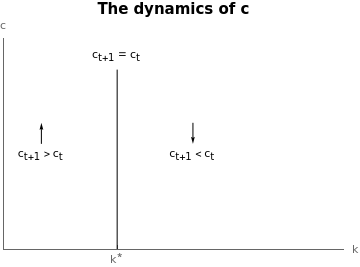
\includegraphics{/home/eric/eric-roca.github.io/static/img/ramsey/dynamics_c.png}
\caption{dynamics of c}
\end{figure}

The arrows show the direction in which consumption \(c\) evolves. As
discussed before, consumtion raises when capital is below \(k^{\star}\)
and raises when above. Note the vertical line: it denotes the level of
capital \(k^{\star}\) such that \(c\) is constant. The value
\(k^{\star}\) can be easily computed:
\(k^{\star} = {f^{\prime}}^{-1}\left(\frac{1-\beta (1-\delta)}{\beta}\right).\)

\hypertarget{the-dynamics-of-k}{%
\subsection{\texorpdfstring{The dynamics of
\(k\)}{The dynamics of k}}\label{the-dynamics-of-k}}

We can proceed simiarly with the motion of capital. The relevant
equation in this case is:

\[k_{t+1} = f(k_{t}) + (1- \delta)k_{t} - c_{t}.\]

As before, we are interested by the combinations of \((k,c)\) such that
capital remains constant over time. In this case, though, and
contrasting with the previous, we will obtain that both capital and
consumption affect capital levels in the future: production uses current
capital, and current consumption depletes current production. We can
rearrange the previous equation to obtain the following:

\[k_{t+1} - k_{t} = f(k_{t}) - \delta k_{t} - c_{t}.\] Setting
\(k_{t+1} = k_{t} \implies k_{t+1} - k_{t} = 0\) so capital is constant
yields:

\[ 0 = f(k_{t}) - \delta k_{t} - c_{t} \implies c_{t} = f(k_{t}) - \delta k_{t}.\]

In the \((k,c)\) space, the equation takes a form similar to a parabola:
it combines production ---with decreasing marginal returns--- with a
linear depreciation rate. Technically, it can be seen that
\(\frac{\partial f(k) - \delta k}{\partial k} = f^{\prime}(k) - \delta\),
which admits a unique maximum: \(f^{\prime}(k)\) is a decreasing
function. Moreover,
\(\frac{\partial^{2} f(k) - \delta k}{\partial k^{2}} = f^{\prime \prime}(k) < 0,\)
confirming that the optimal point is a maximum.

Let's now analyse how capital evolves when consumption is above and
below the level that makes it constant. From
\(k_{t+1} - k_{t} = f(k_{t}) - \delta k_{t} - c_{t}\), if consumption is
above the level we have that \(k_{t+1} - k_{t} < 0,\) meaning that
capital decreases over time. The opposite applies when consumption is
below the level that guarantees a constant level of capital. The Figure
below summarises these findings:

\begin{figure}
\centering
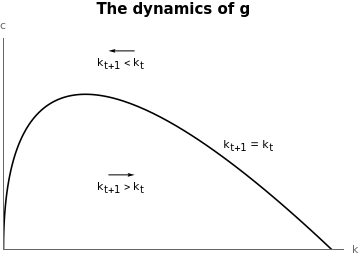
\includegraphics{/home/eric/eric-roca.github.io/static/img/ramsey/dynamics_g.png}
\caption{dynamics of g}
\end{figure}

\hypertarget{the-phase-diagram}{%
\subsection{The phase diagram}\label{the-phase-diagram}}

We can combine the information above to produce the \emph{phase
diagram}. It indicates the motion of variables at different points of
the \((k,c)\) space.

\begin{figure}
\centering
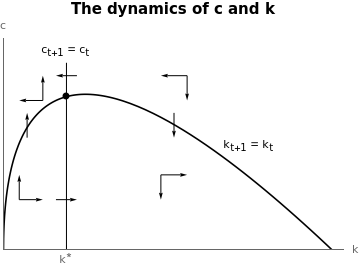
\includegraphics{/home/eric/eric-roca.github.io/static/img/ramsey/phase_diagram.png}
\caption{phase diagram}
\end{figure}

The arrows show the motion of each variable at different conbinations of
\((k,c).\) For instance, to the left of the \(c_{t+1} = c_{t}\) locus
and above the \(_{t+1} - k_{t} = 0\) locus consumption increases and
capital decreases. On top of each curve only capital or consumption
moves, the other remains constant. For example, on the
\(c_{t+1} - c_{t}\) locus, consumption is constant but capital changes.
Finally, the point indicating the intersection of both curves is the
steady state: all variables remain constant at their values. --- title:
Additional material - trajectory linktitle: Trajectory toc: true type:
docs date: ``2019-07-11T00:00:00Z'' lastmod: ``2019-07-11T00:00:00Z''
draft: false menu: Ramsey: parent: The Ramsey model weight: 6

\hypertarget{prevnext-pager-order-if-docs_section_pager-enabled-in-params.toml-1}{%
\section{\texorpdfstring{Prev/next pager order (if
\texttt{docs\_section\_pager} enabled in
\texttt{params.toml})}{Prev/next pager order (if docs\_section\_pager enabled in params.toml)}}\label{prevnext-pager-order-if-docs_section_pager-enabled-in-params.toml-1}}

\hypertarget{weight-6}{%
\subsection{weight: 6}\label{weight-6}}

\hypertarget{the-trajectory-around-the-steady-state}{%
\subsection{The trajectory around the steady
state}\label{the-trajectory-around-the-steady-state}}

For the moment, we have established that the model converges towards a
unique steady state following a saddle path. \textbf{Note:} This means
that there is only one combination of inital capital and consumption,
\((k_{0}, c_{0})\), such that the ecomomy converges. Any other initial
value consumption at \(t=0\) (capital is pre-determined and thus we
\emph{cannot} change it) has a diverging trajectory.

We now compute the exact behaviour of \((k_{t}, c_{t})\) around the
steady state. In general, though, the notion of \emph{around the steady
state} is quite generous and we extend it quite far from the steady
state.

The model is higgly non-linear, so we study a simplied linearised
version around the steady state. First, let's approximate the dynamics
of capital and consumption {[}around the steady state.{]}

\hypertarget{the-approximation-around-the-steady-state}{%
\subsubsection{The approximation around the steady
state}\label{the-approximation-around-the-steady-state}}

The behaviour of the dynamical system around the steady state can be
approximated using a first-order Taylor expansion around it. In that
sense:

\[\begin{pmatrix}
c_{t+1} - \bar{c} \\\ k_{t+1} - \bar{k}
\end{pmatrix}
\approx
\bar{A}
\begin{pmatrix}
c_{t} - \bar{c} \\\ k_{t} - \bar{k}
\end{pmatrix}.\]

This dynamics are governed by 2--dimensional system of difference
equations. To solve it, we begin by studying a simpler system.

\hypertarget{diagonalising-the-matrix-eigenvalues-and-eigenvectors}{%
\subsubsection{Diagonalising the matrix: eigenvalues and
eigenvectors}\label{diagonalising-the-matrix-eigenvalues-and-eigenvectors}}

\textbf{Note:} based on the notes by
\href{http://www.princeton.edu/~moll/ECO503Web/Lecture4_ECO503.pdf}{Benjamin
Moll}.

To simplify notation, let
\(y_{t} = \begin{pmatrix} c_{t} - \bar{c} \\\ k_{t} -\bar{k} \end{pmatrix}.\)
Our problem can be written as: \(y_{t+1} = \bar{A} y_{t}\).

It \(\bar{A}\) was a diagonal matrix, the solution to the system would
be straighforward. In fact, if that were the case (I change variables to
avoid confussion):

\[\begin{pmatrix} \phi_{t+1} \\\\ \omega_{t+1} \end{pmatrix} = \begin{pmatrix} a_{1,1} & 0 \\\ 0 & a_{2,2} \end{pmatrix} \begin{pmatrix} \phi_{t} \\\ \omega_{t} \end{pmatrix}.\]
Then, it is clear that
\(\phi_{t+1} = a_{1,1} \phi_{t} \implies \phi_{t} = a_{1,1}^{t} \phi_{0}.\)
And we would find a similar, equivalent expression for \(\omega.\)

\(\bar{A}\) is not diagonal, but we can apply a Jordan decomposition to
it and obtain an equivalent system governed by a diagonal matrix. In
particular, we look for an \(2 \times 2\) invertible matrix \(X\) such
that \( X^{-1} \Lambda X = \bar{A}\), where \(\Lambda\) is
diagonal. Then, we apply the following transformation to our system
(pre-mulitiplying by \(\color{red}{X^{-1}}\) on both sides and
multiplying by \(\color{green}{XX^{-1}}\) on the righ-hand side).
\[ \color{red}{X^{-1}} y_{t+1} = \color{red}{X^{-1}} \bar{A} \color{green}{(X X^{-1})} y_{t} = X^{-1} y_{t+1} = X^{-1} \bar{A} X (X^{-1} y_{t}) =\]
\[ = \Lambda X^{-1} y_{t}.\]

Denote \(z \equiv X^{-1} y\). Thus, the system becomes:

\[z_{t+1} = \Lambda z_{t}.\] Since \(\Lambda\) is diagonal, the soltions
are of the form: \[z_{t} = \Lambda^{t} z_{0}.\] \textbf{Note:} in
general, the power of a matrix is complex. However, for a \emph{diagonal
matrix} it is simply the power of each component.

Once we have the solution for the transformed system we must undo the
transformation: in fact, we do not care abut the evolution of \(z\).
This step involves using that \(X^{-1} y = z \implies y = X z\).

\hypertarget{the-matrix-lambda}{%
\paragraph{\texorpdfstring{The matrix
\(\Lambda\)}{The matrix \textbackslash{}Lambda}}\label{the-matrix-lambda}}

In a Jordan decomposition, the diagonal matrix \(\Lambda\) consists of
the matrix whose entries are its eigenvalues. Thus (we have a
\(2 \times 2\) system), \[\Lambda = \begin{pmatrix} 
    \lambda_{1} & 0  \\\
    0 & \lambda_{2} 
\end{pmatrix}.\]

\hypertarget{the-matrix-x}{%
\paragraph{\texorpdfstring{The matrix
\(X\)}{The matrix X}}\label{the-matrix-x}}

The matrix \(X\) contains the eigenvectors of \(\bar{A}\) in columns.
There is one eigenvector associated to each eigenvalue. \textbf{Note:}
it is important to correctly relate each eigenvetor to its eigenvalue.

To find an eigenvector associated with \(\lambda_{1}\) (\emph{there are
infinitely many possible eigenvectors, we only want one}) we solve the
following system:

\[\bar{A} \begin{pmatrix} v_{1} \\\ v_{2} \end{pmatrix} = \lambda_{1} \begin{pmatrix} v_{1} \\\ v_{2} \end{pmatrix} \quad \mathrm{or} \quad (\bar{A} - \lambda_{1} \mathbb{I}) 
\begin{pmatrix} v_{1} \\\ v_{2} \end{pmatrix} = \begin{pmatrix} 0 \\\ 0 \end{pmatrix}.\]

The matrix \(X\) then becomes:

\[X = \begin{pmatrix} v_{1,1} & v_{2,1} \\\ 1 & 1 \end{pmatrix}.\]

\hypertarget{solving-the-system}{%
\subsubsection{Solving the system}\label{solving-the-system}}

We begin with the solution for the transformed variable \(z.\) We
already know its takes the form:

\[z_{t} = \Lambda^{t} z_{0} \quad \mathrm{or} \quad \begin{pmatrix} z_{t}^{1} \\\ z_{t}^{2} \end{pmatrix} = \begin{pmatrix} \lambda_{1}^{t} & 0 \\\ 0 & \lambda_{2}^{t} \end{pmatrix} \begin{pmatrix} v_{0}^{1} \\\ v_{0}^{2} \end{pmatrix}.\]

Next, we reverse the transformation, this is, we obtain the dynamics of
\(y: y_{t} = X z_{t}.\) Therefore, we obtain:

\[y_{t} = X z_{t} = X \Lambda^{t} z_{0} = \begin{pmatrix} v_{1,1} & v_{2,1} \\\ v_{1,2} & v_{2,2} \end{pmatrix} \begin{pmatrix} \lambda_{1}^{t} & 0 \\\ 0 & \lambda_{2}^{t} \end{pmatrix} \begin{pmatrix} z_{0}^{1} \\\ z_{0}^{2} \end{pmatrix}.\]

Alternatively, multiplying the matrices and recalling that
\(y_{t}=\begin{pmatrix} c_{t} - \bar{c} \\\ k_{t} - \bar{k} \end{pmatrix}\)
:

\[\begin{pmatrix} c_{t} - \bar{c} \\\ k_{t} - \bar{k} \end{pmatrix} = z_{0}^{1} \lambda_{1}^{t} \begin{pmatrix} v_{1,1} \\\ v_{1,2} \end{pmatrix} + z_{0}^{2} \lambda_{2}^{t} \begin{pmatrix} v_{2,1} \\\ v_{2,2} \end{pmatrix}.\]

The eigenvalues appear clearly in the solution. \textbf{Remember} that
we know that one eigenvalue is bigger than one, while the second lies
within the unit circle. Without lose of generality, assume that
\(\lambda_{1} \in (-1,1)\) and \(\lambda_{2} > 1.\) According to the
solution before, this implies an explosive behaviour:
\(\lambda_{2} > 1 \implies \lim_{t \rightarrow +\infty} \lambda_{2}^{t} = +\infty.\)
To have a well-behaved dynamics we must impose \(z_{0}^{2} = 0\), which
eliminates the explosive behaviour.

\textbf{Technical remark:} Denote by \(l\) the number of eigenvalues in
the unit circle, and denote by \(m\) the number of pre-determinted state
variables:

\begin{itemize}
\tightlist
\item
  if \(l=m\) (standard case): saddle-path, \emph{unique} optimal
  trajectory. The eigenvalues within the unit circle govern the speed of
  convergence.
\item
  if \(l < m\): unstable
\item
  if \(l > m\): multiple optimal trajectories.
\end{itemize}

After imposing \(z_{0}^{2} = 0\) the system becomes:

\[\begin{pmatrix} c_{t} - \bar{c} \\\ k_{t} - \bar{k} \end{pmatrix} = z_{0}^{1} \lambda_{1}^{t} \begin{pmatrix} v_{1,1} \\\ v_{1,2} \end{pmatrix}.\]

\hypertarget{closing-the-model-with-initial-values}{%
\paragraph{Closing the model with initial
values}\label{closing-the-model-with-initial-values}}

We know that the economy begins with a level of capital
\(k_{t=0} = k_{0} > 0.\) Substituting \(t=0\) in the equation above, and
focusing on capital, we obtain:

\[k_{0} - \bar{k} = z_{0}^{1} v_{1,2} \implies \color{red}{z_{0}^{1} = \frac{k_{0} - \bar{k}}{v_{1,2}}}.\]
Therefore, we can substitute the value for \(z_{0}^{1}\) to obtain the
dynamics of capital:

\[k_{t} - \bar{k} = \color{red}{z_{0}^{1}} \lambda_{1}^{t} v_{1,2} = \left(k_{0} - \bar{k} \right) \lambda^{t}.\]

Similarly, we have that for consumption:

\[c_{t} - \bar{c} = \color{red}{z_{0}^{1}} \lambda_{1}^{t} v_{1,1} = \frac{v_{1,1}}{v_{1,2}} \lambda_{1}^{t} (k_{0} - \bar{k}).\]
Finally, the initial value of consumption \(c_{0}\) that puts the
economy in the saddle path is obtained by setting \(t=0\) in the
previous equation:

\[c_{0} - \bar{c} = \frac{v_{1,1}}{v_{1,2}} (k_{0} - \bar{k}).\]

We can now completely solve an example.

\hypertarget{utility-and-production-functions}{%
\subsection{Utility and production
functions}\label{utility-and-production-functions}}

We assume that utility is logarithmic and we take a Cobb-Douglas
production function.

\begin{eqnarray}
u(c_{t}) = \log (c_{t}), \\\
F(K_{t},X_{t}) = AK_{t}^{\alpha}X_{t}^{1-\alpha}, \\\
A >0, \alpha \in (0,1).
\end{eqnarray} \$\$ We can check that both functions satisfy the Inada
conditions:

\[\lim_{c_{t} \rightarrow 0}u^{\prime}(c_{t}) = \lim_{c_{t} \rightarrow 0} \frac{1}{c_{t}} = +\infty, \\\
  \lim_{c_{t} \rightarrow +\infty}u^{\prime}(c_{t}) = \lim_{c_{t} \rightarrow +\infty} \frac{1}{c_{t}} = 0, \\\
  \lim_{K_{t} \rightarrow 0} F^{\prime}_{K_{t}}(K_{t}, X_{t}) = \lim_{K_{t} \rightarrow 0} A\alpha K_{t}^{\alpha - 1}X_{t}^{1-\alpha} = +\infty, \\\
  \lim_{K_{t} \rightarrow +\infty} F^{\prime}_{K_{t}}(K_{t}, X_{t}) = \lim_{K_{t} \rightarrow +\infty} A\alpha K_{t}^{\alpha - 1}X_{t}^{1-\alpha} = 0, \\\
  \lim_{X_{t} \rightarrow 0} F^{\prime}_{X_{t}}(K_{t}, X_{t}) = \lim_{X_{t} \rightarrow 0} A (1-\alpha) K_{t}^{\alpha}X_{t}^{\alpha} = +\infty, \\\
  \lim_{X_{t} \rightarrow +\infty} F^{\prime}_{X_{t}}(K_{t}, X_{t}) = \lim_{X_{t} \rightarrow +\infty} A (1- \alpha) K_{t}^{\alpha}X_{t}^{\alpha} = 0.
\]

The production function, expressed in intensive terms, becomes:

\[F(K_{t}, X_{t}) = X_{T} F\left(\frac{K_{t}}{X_{t}},1\right) = X_{t} f(k_{t}) = X_{t} k_{t}^{\alpha}, k_{t} \equiv \frac{K_{t}}{X_{t}}.\]
with total production \(Y_{t} = F(K_{t},X_{t})\) and production per
capita equal to \(y_{t} \equiv \frac{Y_{t}}{X_{t}} = f(k_{t}).\)

\hypertarget{households-optimisation}{%
\subsection{Household's optimisation}\label{households-optimisation}}

Instead of using the results from previous sections, we develop again
the utility maximisation. First, we write down the household's budget
constraint:

\hypertarget{households-budget-constraint-1}{%
\subsubsection{Household's budget
constraint}\label{households-budget-constraint-1}}

At each period, total received income is composed of \emph{wages} and
\emph{interests}. It can be spend on \emph{consumption} or
\emph{saving}. Remember that capital depreciates at a rate
\(\delta \in [0,1].\) Hence, we receive back from firms \(1-\delta\)
times the capital we lend. Therefore:

\[ w_{t} + r_{t}k_{t} + (1-\delta)k_{t} = c_{t} + k _{t+1}.\]

\hypertarget{intertemporal-utility-maximistion-lagrangean}{%
\subsubsection{Intertemporal utility maximistion:
Lagrangean}\label{intertemporal-utility-maximistion-lagrangean}}

The intertemporal utility maximisation problem is:

\begin{eqnarray}
\max_{c_{t}, k_{t+1}}  \sum_{t=0}^{\infty} \beta^{t} u(c_{t}) & \\\
\mathrm{s.t.} \quad      w_{t} + r_{t} k_{t} + (1-\delta)k_{t} = c_{t} + k_{t+1}, \\\
         c_{t}, k_{t+1} >0, k_{t=0} = k_{0} > 0.
\end{eqnarray} \$\$

The Lagrangean becomes:

\[ \mathcal{L} = \sum_{t=0}^{\infty} \beta^{t} u(c_{t}) + \sum_{t=0}^{\infty} \lambda_{t}(w_{t} + (r_{t} + 1 - \delta)k_{t} - c_{t} - k_{t+1}).\]

We use the first-order conditions with respect to \(c_{t}\) and
\(k_{t+1}\) to find the optimal consumption path. In particular, in this
step we shall obtain the Euler equation, which we combine latter with
the transversality condition.
\[ \frac{\partial \mathcal{L}}{\partial c_{t}} = \beta^{t} u^{\prime}(c_{t}) - \lambda_{t} = \beta^{t}\frac{1}{c_{t}} - \lambda_{t} = 0 \\\
   \frac{\partial \mathcal{L}}{\partial k_{t+1}} = -\lambda_{t} + \lambda_{t+1} (r_{t+1} + 1 - \delta) = 0.
\] \textbf{Note:} the term \(k_{t+1}\) appears within the summation at
\(t=t+1.\) In fact expanding it reveals this fact clearly:
\[ + \ldots \lambda_{t} (w_{t} + (r_{t} + 1 - \delta)k_{t} - c_{t} - k_{t+1}) + \\\
   \quad \quad + \lambda_{t+1}(w_{t+1} + (r_{t+1} + 1 - \delta)k_{t+1} - c_{t+1} - k_{t+2} + \ldots\]

Combining both, we obtain the Euler equation:

\[\beta^{t}\frac{1}{c_{t}} = r_{t+1} \beta^{t+1} \frac{1}{c_{t+1}} \implies c_{t+1} = \beta (r_{t} + 1 - \delta)c_{t}.\]

Finally, we should remember to impose the transversality condition:

\[\lim_{t \rightarrow +\infty} \beta^{t}u^{\prime}(c_{t})k_{t+1} = \lim_{t \rightarrow +\infty}\beta^{t}\frac{1}{c_{t}k_{t+1}} = 0.\]

\hypertarget{firms-optimisation}{%
\subsection{Firm's optimisation}\label{firms-optimisation}}

In this model, firms operate under pefect competition, making zero
profits. Moreover, factors are paid their marginal productivity.

\[r_{t} = F^{\prime}_{K_{t}}(K_{t}, X_{t}) = \alpha K_{t}^{\alpha - 1}X_{t}^{1-\alpha} = \alpha \left(\frac{K_{t}}{X_{t}}\right)^{\alpha - 1} = \alpha k_{t}^{\alpha -1}. \\\
  w_{t} = F^{\prime}_{X_{t}}(K_{t}, X_{t}) = (1-\alpha) K_{t}^{\alpha} X_{t}^{-\alpha} = (1-\alpha)\left(\frac{K_{t}}{X_{t}}\right)^{\alpha} = (1-\alpha) k_{t}^{\alpha}.\]

Alternatively, using the information in the {[}Appendix{]} and working
directly with the intensive-form production function:

\[r_{t} = f^{\prime}(k_{t}) = \frac{\partial f(k_{t})}{\partial k_{t}} = \alpha k_{t}^{\alpha -1}, \\\
  w_{t} = f(k_{t}) - f^{\prime}(k_{t})k_{t} = k_{t}^{\alpha} - \alpha k_{t}^{\alpha - 1} k_{t} = (1-\alpha)k_{t}^{\alpha}.\]

\hypertarget{the-dynamic-system}{%
\subsection{The dynamic system}\label{the-dynamic-system}}

We are now in a position to solve the model. We have the following
equations:

\[ c_{t+1} = \beta (r_{t+1} + 1 - \delta) c_{t}, \\\
   w_{t} + r_{t}k_{t} + (1-\delta) k_{t} = c_{t} + k_{t+1}, \\\
   w_{t} = (1-\alpha) k^{\alpha}_{t}, \\\
   r_{t} = \alpha k^{\alpha-1}, \\\
   \lim_{t \rightarrow +\infty} \beta^{t}\frac{1}{c_{t}} k_{t+1} = 0.\]

Substituing the wage and interest rate into the budget constraint allows
us to retrieve the dynamics of capital:

\[ c_{t+1} = \beta (\alpha k^{\alpha-1} + 1 - \delta) c_{t}, \\\
   k_{t}^{\alpha} + (1-\delta) k_{t} = c_{t} + k_{t+1}, \\\
   \lim_{t \rightarrow +\infty} \beta^{t}\frac{1}{c_{t}} k_{t+1} = 0.\]

\hypertarget{steady-state}{%
\subsubsection{Steady state}\label{steady-state}}

Before trying to solve for the optimal trajectory, we analyse the steady
states of this economy. A steady-state \((\bar{k}, \bar{c}\) is such
that capital and consumption remain constant over time:
\(c_{t+1} = c_{t}\) and \(k_{t+1} = k_{t}.\) Applying this idea to the
equations above we get ---here we can temporarily forget about the
transversality condition.

\[ \bar{c} = \beta(\alpha \bar{k}^{\alpha-1} + 1 - \delta) \bar{c}, \\\
   \bar{k}^{\alpha} + (1-\delta)\bar{k} = \bar{c} + \bar{k}.\]

Hence, using the first equation we can easily get the steady level of
capital:
\[ \bar{k} = \left(\frac{\alpha \beta}{1-\beta(1-\delta)}\right)^{\frac{1}{1-\alpha}}.\]
Using this solution in the second equation yields the steady-state level
of consumption:
\[ \bar{c} = \left(\frac{\alpha \beta}{1-\beta (1-\delta)}\right)^{\frac{\alpha}{1-\alpha}} - \delta \left(\frac{\alpha \beta}{1-\beta (1- \delta)}\right)^{\frac{1}{1-\alpha}}.\]

\hypertarget{stability-1}{%
\subsection{Stability}\label{stability-1}}

First, we analyse the stability of the steady state, as we did in the
{[}general case{]} Since we are using log-utility, the coefficient of
relative risk aversion \(\epsilon_{c} = 1.\)

Instead of plugging the correct values in the Jacobian matrix
\(\bar{A}\), for the sake of clarity, we derive everything again:

\[\bar{A} = \begin{pmatrix}
\frac{\partial c_{t+1}}{\partial c_{t}} & \frac{\partial c_{t+1}}{\partial k_{t}} \\\
\frac{\partial k_{t+1}}{\partial c_{t}} & \frac{\partial k_{t+1}}{\partial k_{t}}
\end{pmatrix}
\] \[ = \] \[\begin{pmatrix}
\beta \left( \alpha k_{t+1}^{\alpha -1} + 1 - \delta \right) - \frac{\beta c_{t} \alpha (\alpha-1) }{k_{t+1}^{2-\alpha}} & \frac{\beta c_{t} \alpha (\alpha -1)}{k_{t+1}^{2-\alpha}} \left( \alpha k_{t}^{\alpha-1} + 1 - \delta \right) \\\
-1 & \alpha k_{t}^{\alpha -1} + 1 - \delta \end{pmatrix}\]

Evaluating it at the steady state: \[\bar{A}\bigr\rvert_{\substack{
    k_{t} = k_{t+1} = \bar{k} \\\
     c_{t} = c_{t+1} = \bar{c}
}
}
   = \begin{pmatrix}
    1 - \beta \bar{c}  \alpha (\alpha -1) \bar{k}^{\alpha -2}  & \alpha (\alpha -1 ) \bar{c}  \bar{k}^{\alpha -2} \\\
    -1  & \frac{1}{\beta}
\end{pmatrix},\]

where we have used
\(1 = \beta \left( \alpha \bar{k}^{\alpha -1} + 1 - \delta \right)\) at
the steady state.

We can use the fact
\(\mathrm{tr}(\bar{A}) = \lambda_{1} + \lambda_{2}, \mathrm{det}(\bar{A}) = \lambda_{1} \lambda_{2}.\)
Therefore:

\[\lambda_{1} \lambda_{2} = \frac{1}{\beta} \]
\[\lambda_{1} + \lambda_{2} = \frac{1}{\beta} + 1 - \beta \bar{c} \alpha (\alpha-1) \bar{k}^{\alpha -2}.\]
The first equation implies that either a)
\(\lambda_{1} > 0, \lambda_{2} > 0\) or b)
\(\lambda_{1} < 0, \lambda_{2} < 0.\) However, since
\(\lambda_{1} + \lambda_{2} > 1\) b) is impossible. Then,
\(\lambda_{1} > 0, \lambda_{2} > 0.\) Substitute \(\lambda_1 \lambda_2 = \frac{1}{\beta} \) in the second equation:

\[ \lambda_{1} + \lambda_{2} = 1+ \lambda_{1} \lambda_{2} - \beta ( \alpha (\alpha - 1) \bar{k}^{\alpha -2}\frac{\bar{c}}{\epsilon_{\bar{c}}}.\]

Rearranging:
\[ \lambda_{1} + \lambda_{2} - \lambda_{1} \lambda_{2} =  1+  - \beta \alpha (\alpha -1) \bar{k}^{\alpha -2}\frac{\bar{c}}{\epsilon_{\bar{c}}} > 1 \implies \lambda_{1} + \lambda_{2} - \lambda_{1}\lambda_{2} - 1 >0.\]
Factorisation leads to: \[(1 - \lambda_{2})(\lambda_{1} - 1) > 0.\]
Therefore: \[ \lambda_{2} < 1 \] \[ \lambda_{1} > 1 \]
\[ \lambda_{1} > 0, \lambda_{2} > 0\] and \textbf{the steady state is
saddle.}

\hypertarget{trajectory}{%
\subsection{Trajectory}\label{trajectory}}

Describing the trajectory around the steady state analitycally would be
cumbersome. Introducing an alternative production function of the \(Ak\)
family alleviates this problem, see the notes by
\href{https://eml.berkeley.edu/~webfac/obstfeld/e202a_f13/lecture2.pdf}{Maurice
Obsfeld}

Instead, we solve this section numerically. In particular, assume that
\(\alpha = 0.3, \\, \beta = 0.9, \\, \delta = 0.1.\) The initial level
of capital \(k_{t=0} = 1.\)

With these values, we have the following:

\[\bar{k} = 1.65202, \\, \bar{c}=0.997329, \\, \bar{A} = \begin{pmatrix} 1.08029 & -0.089214 \\\ -1 & 1.11111 \end{pmatrix}.\]

The eigenvalues of the matrix \(\bar{A}\) are
\[\lambda_{1} = 0.796618 \in (-1,1)\] \[\lambda_{2} =1.39479 > 1.\]

One possible set of eigenvectors is given by:

\[v_{1} = (0.314494 , 1), v_{2} = (-0.283675, 1)\] which are associated
to \(\lambda_{1}\) and \(\lambda_{2}\), respectively. Hence, the matrix

\[X = \begin{pmatrix} 0.314494 & -0.283675 \\\ 1 & 1 \end{pmatrix}.\]

\hypertarget{solving-the-system-1}{%
\subsubsection{Solving the system}\label{solving-the-system-1}}

Applying the results from before the system is:

\[\begin{pmatrix} c_{t} - \bar{c} \\\ k_{t} - \bar{k} \end{pmatrix} = z_{0}^{1} 0.796618^{t} \begin{pmatrix} 0.314494 \\\ 1 \end{pmatrix} + z_{0}^{2} 1.39479 \begin{pmatrix} -0.283675 \\\ 1 \end{pmatrix}.\]

Since \(\lambda_{2} > 1\) we must set the value \(z_{0}^{2} = 0\) to
avoid an explosive behaviour. Consequently:

\[\begin{pmatrix} c_{t} - \bar{c} \\\ k_{t} - \bar{k} \end{pmatrix} = z_{0}^{1} 0.796618^{t} \begin{pmatrix} 0.314494 \\\ 1 \end{pmatrix}.\]

We can solve the equation first by setting \(t=0\) to obtain the value
\(z_{0}^{1}:\)

\[\underbrace{k_{0}}_{=1} - \underbrace{\bar{k}}_{=1.65202} =  z_{0}^{1} \times 1= -0.652017.\]

Consequently, the dynamic equation for capital becomes:

\(k_{t} - \bar{k} = -0.652017 \times 0.796618^{t}\)

And for consumption:

\(c_{t} - \bar{c} = -0.652017 \times 0.314494 \times 0.796618^{t} = -0.205055 \times 0.786618^{t}.\)
Finally, we solve for the initial level of consumption compatible with
the saddle path. For \(t=0\) we have:

\(c_{0} - \underbrace{\bar{c}}_{=0.997329} = \underbrace{z_{0}^{1}}_{= -0.652017} \times 0.314494 \implies c_{0} = 0.792273.\)

\hypertarget{optimality}{%
\subsection{Optimality}\label{optimality}}

Before {[}we claimed{]} that the solution is \emph{optimal} despite the
fact that it does not maximise consumption at the steady state. However,
what we claimed was that the \emph{entire path} was optimal. We can
proof it solving the Ramsey allocation problem from the perspective of
the social planner.

\hypertarget{social-planner}{%
\subsubsection{Social planner}\label{social-planner}}

A social planner maximises total welfare, given by:

\[\max \sum_{t=0}^{\infty} \beta^{t} u(c_{t}).\]

The social planner directly allocates resource between consumption and
investment, so he is not bothered by wages or interest rates. Hence, his
intertemporal budget constraint reads. In particular, he has to allocate
total production and capital net of depreciation between \(c_{t}\) and
\(k_{t+1}.\)

\[f(k_{t}) = c_{t} + k_{t+1} + (1-\delta) k_{t}.\] He operates under a
certain level \(k_{0} > 0\) given.

Note how the budget constraint is equivalent to the one we found in the
competitive equilibrium. Moreover, total welfare coincides, too. Hence,
the solutions will be the same, proving that the competitive equilibrium
was optimal.

The two main equations of the model are relevant for the planner as
well. First, he must follow the Euler equation. In fact, he can reduce
present consumption by \(\Delta c\) at time \(t\) and save it. The
present-day cost is \(u^{\prime} ( c_{t} ) \Delta_{c}\). He obtainins
\(f^{\prime}(k_t) \Delta_{c} + (1-\delta) \Delta_{c}\) at time \(t+1,\)
which raises utility by
\(\left( f^{\prime}(k_{t}) \Delta_{c} + (1-\delta) \Delta_{c} \right) u^{\prime}_{c_{t+1}}.\)
Optimality implies that this trade off is not possible anymore, hence,
we obtain the Euler equation again.

Secondly, although the planner directly allocates consumption and
investments, he must follow the technological constraint displayed
above. This does not represent preferences, and coincides with the
househld's budget constraint after clearing the markets.

Finally, observe that the \emph{first welfare theorem} directly applies:
if markets are competitve and there re no externalities, then the
decentralised equilibrium is Pareto-efficient. All conditions hold in
the Ramsey model.

\hypertarget{the-golden-rule}{%
\subsection{The Golden rule}\label{the-golden-rule}}

We have discussed before that, in the Ramsey model, the economy
converges to a steady state with \(\bar{k}\) below the golden-rule level
of capital \(k^{\mathcal{GR}}\).

This constrasts with the Solow model: in the Solow model, a sufficietly
high saving rate causes capital over-accumulation. This opens the
possibility of finding alternative paths that yield higher consumption
levels in each and every period ---meaning that such a saving rate was
not Pareto-efficient.

In the Ramsey model, savings are optimally derived from the utility
maximisation, and the level of utility depends on consumption. Moreover,
the model features \emph{no} externalities. Consequently, the model
cannot produce a situation whereby it is possible to increase
consumption at each and every period: this contradicts optimisation.

However, \(\bar{k} < k^{\mathcal{GR}}\) implies that it is possible to
increase the saving rate today, build up the extra capital needed to
reach \(k^{\mathcal{GR}}\) and then be able to consume
\(c^{\mathcal{GR}} > \bar{c}\) at the steady state ---which, remember,
lasts forever. Suppose that we had reached the steady-state. Why do the
households not change their saving rate to reach \(c^{\mathcal{GR}}?\)
The reason is that households value present consumption more than future
consumption. Therefore, the current utility cost of a reduction in
consumption is larger the future gains once discounted. Because of the
discount rate, the utility gains from an eventual permanent increase in
consumption are bounded.

All in all, the economy converges to a value \(\bar{k}\) below the
steady state. Because \(\bar{k}\) is the optimal level of \(k\) for the
economy to converge to, it is known as the \emph{modified golden-rule}
capital stock.

We {[}had already noticed{]} that the discount factor \(\beta\) prevents
the economy from reaching the golden-rule level of captal. According to
our computation, the Golden-rule level of capital is only attained if
\(\beta = 1.\) This implies that present and future consumption are
valued the same, which complements the discussion above.
\end{document}
